\chapter{量子力学与Morse理论}
Morse理论是几何上的重要定理,微分几何中对一个流形我们可以考虑上面的标量场,其微分的定义也是十分自然的。如果在某点$p\in\mathcal{M}$,$(df)|_p=0$,而且这样的点都是孤立点且Hessian矩阵非退化,那么就称这样的函数是Morse函数。而Morse定理是一组不等式,告诉我们这些微分为0的点的个数看似是流形局部的性质,其实是由流形的整体拓扑决定的。后面会详细介绍这一理论,我们先考虑一个最简单的例子。考虑一个可定向二维闭曲面$gT^2$,Hessian矩阵不退化,那么可以根据Hessian矩阵正负本征值个数把函数微分为0的点分类为极大值、极小值和鞍点。Morse定理告诉我们:
\begin{equation}
	\begin{cases}
		\text{极大值点的个数}&\geq 1\\
		\text{极小值点的个数}&\geq 1\\
		\text{鞍点的个数}&\geq 2g
	\end{cases}
\end{equation}
前面两个不等式其实是在说流形的连通分支个数是1,也是流形整体的性质。这个定理显然是可以从纯数学的角度来证明的,但是Witten在1982年对这一理论给出了(超对称)量子力学版本的证明\cite{Witten:1982im},这一角度十分之有趣,后面讲会从比较偏重于数学的角度来考虑这一证明。
\section{量子力学基础}
本节的目的差不多是量子力学补遗,看下数学家思考量子力学的角度。
\subsection{Wyle算符}
量子力学里面所谓量子化就是把力学量从函数变成算符:
\begin{equation}
	\{f,g\}\Rightarrow\{\hat f,\hat g\}_q=\frac{1}{i\hbar }[\hat f,\hat g]
\end{equation}
这里$\{\cdot\}$是经典Poisson括号,下标$q$表示对应量子化后的量子泊松括号,它和对易子成正比。当我们用哈密顿形式,把动力学方程完全用Possion括号的形式写出来,然后全部做了这样的替换之后量子化也就完成了。而量子力学基本假设里面很重要的一条是量子化之后位置和动量算符不对易,这导致在涉及到$f(x,p)=x^mp^n$的力学量量子化时会出现定义模糊。实际上这一问题解决有很多种方案,我们采取从数学角度上讲比较好的方法。

在位置表象下考虑,这时$\hat x\to x,\hat p\to-i\hbar\partial_x$,考虑力学量$f(x,p)=\sum_m f_m(x)p^m$,尝试下面两种极端的量子化方案,作用在任意一个函数$v(x)$上为:
\begin{equation}
	\begin{aligned}
		&f^+v =\sum_m f_m(x)\left(-i\hbar\partial_x\right)^m v(x)=\sum_m \left.\left(-i\hbar\partial_x\right)^m f_m(y)v(x)\right|_{y=x}\\
		&f^-v =\sum_m \left(-i\hbar\partial_x\right)^m \left[f_m(x)v(x)\right]=\sum_m \left.\left(-i\hbar\partial_x\right)^m f_m(x)v(x)\right|_{y=x}
	\end{aligned}
\end{equation}
Wyle算符就定义称折中的方案:
\begin{equation}
	\hat f_{\text{Wyle}} v \equiv \sum_m \left.\left(-i\hbar\partial_x\right)^m f_m\left(\frac{x+y}{2}\right)v(x)\right|_{y=x}
\end{equation}
这样做量子化会让半经典极限,也就是$\hbar\to 0$的极限性质比较好。

\begin{theorem}[半经典极限]
	$\hbar \to 0$,有:
	\begin{equation}
		\hat f \hat g=\widehat{fg}+\mathcal{O}(\hbar),\quad\left\{\hat f,\hat g\right\}_q=\widehat{\left\{f,g\right\}}+\mathcal{O}(\hbar)
	\end{equation}
\end{theorem}
\begin{proof}
 	使用数学归纳法进行证明,
\end{proof}

\subsection{一维散射问题}
考虑一个在$[x_1,x_2]$内才不为0的势场,入射波能量$E>0$。量子力学对这个问题已经充分的研究过了,我们只需在平面波边界条件下求解下面的薛定谔方程就好:
\begin{equation}\label{7.6}
	-\frac{\hbar^2}{2}\psi^{\prime\prime}+V(x)\psi= E\psi
\end{equation}
其中我们已经选取合适的量纲使得$m=1$。数学上并不是解方程这么玩的,下面我们就来欣赏一下数学家的做法,数学家或许不能告诉你这个微分方程具体的解,但是他却能告诉你非常多的解的性质。首先假设方程\ref{7.6}的解空间为$L$,这是一个二维的函数线性空间。现在考虑$(-\infty,x_1)\cup(x_2,+\infty)$上的薛定谔方程:
\begin{equation}\label{7.7}
	-\frac{\hbar^2}{2}\psi^{\prime\prime}= E\psi
\end{equation}
对应的解空间设为$L_0=\operatorname{span}\{e_1=\sin(kx),e_2=\cos(kx)\}$。则可以定义单值化算子:
\begin{definition}[单值化算子]
	$B_{\pm}:L\to L_0,u(x)\in L,u_0(x)\in L_0$定义:
	\begin{equation}
		\begin{aligned}
			&B_- u (x)=u_0(x),\quad \left.u=u_0\right|_{x<x_1}\\
			&B_+ u (x)=u_0(x),\quad \left.u=u_0\right|_{x>x_2}
		\end{aligned}
	\end{equation}
	根据ode的解唯一存在性定理,可知$B_{\pm}$是同构,下面的单值化算子是well-define的:
	\begin{equation}
		M\equiv B_+B_-^{-1}
	\end{equation}
\end{definition}
熟悉高等量子散射理论的我们立刻就可以看出这里的$B_{\pm}$其实就是Moller算符$\Omega_{\pm}$,而这里的$M$其实就像是散射矩阵$S\equiv\Omega_-^\dagger\Omega_+$。

在$L_0$中选取正弦余弦作为基底,设$\eta\xi\in L_0$,定义下面的楔积,用对易子符号表示\footnote{有点符号混用}:
\begin{equation}
	\left[\xi,\eta\right]\equiv \xi\wedge \eta =\xi_1\eta_2-\xi_2\eta_1
\end{equation}
\begin{theorem}\label{7.1.3}
	$M$保$\left[\cdot,\cdot\right]$不变。$\left[M(\xi),M(\eta)\right]=\left[\xi,\eta\right]$
\end{theorem}
为了证明这个定理我们先证个引理,其中遇到的概念后面也会非常有用。
\begin{definition}[斜积]
	\begin{equation}
		\left\{\psi,\phi\right\}\equiv\psi^\prime\phi-\psi\phi^\prime
	\end{equation}
\end{definition}
这其实就是朗斯基行列式的定义,而且不难证明其不依赖于$x$,是一个常数,也即$\partial_x\left\{\psi,\phi\right\}=0$。
\begin{lemma}
	\begin{equation}
		\{\psi,\phi\}=-k\left[B_\pm\psi,B_\pm\phi\right]
	\end{equation}
\end{lemma}
\begin{proof}
	由于$\{\psi,\phi\}$与$x$无关,所以
	\begin{equation}
			\{\psi,\phi\}=\{\psi,\phi\}_{x<x_1}=k(-\xi_1\eta_2+\xi_2\eta_1)=-k[B_-\psi,B_-\phi]
	\end{equation}
	另一个等式可以通过把上面证明中$x<x_1$换成$x>x_2$就完成了证明。
\end{proof}
现在来证明定理\ref{7.1.3}:
\begin{proof}
	
\end{proof}
\begin{corollary}
	$\det M=1$
\end{corollary}

注意我们到现在为止讨论的都是实值函数空间,实际上量子力学里面更方便的做法是考虑$L_0,L_1$的复化,这样做会方便很多。
\begin{definition}[复化]
	设$V$ 是实向量空间。
	\begin{itemize}
		\item 	$ V$的复化(记作$V_\mathbb{C}$)等于$V\times V$,其元素是有序对 $(u,v)$,其中 $u,v\in V$
		但我们把它写作$u+\mathrm{i}v$。\\
		\item
		定义$V_{\mathbf{C}}$ 上的加法为
		$$(u_1+\mathrm{i}v_1)+(u_2+\mathrm{i}v_2)=(u_1+u_2)+\mathrm{i}(v_1+v_2)$$
		其中$u_1,v_1,u_2,v_2\in V$。\\
		\item
		定义$V_{\mathbb{C}}$上的复标量乘法为
		$$(a+b\text{i})(u+\text{i}v)=(au-bv)+\text{i}(av+bu)$$
		其中$a, b\in \mathbb{R} , \quad u, v \in V$。
	\end{itemize}
	原先实向量空间的算子$T$可自然复化为$T_{\mathbb{C}}$,$T_\mathbb{C}(u+iv)\equiv T(u)+iT(v) $
\end{definition}
\begin{remark}
	这其实涉及到量子力学为什么需要复数,能否构造纯粹在实数空间上定义的量子力学?近年来潘建伟老师组的实验工作否定了这一点\cite{Renou:2021dvp,Chen:2021ril},我从文章\cite{karam_why_2020}的角度来稍微提一下。
\end{remark}

复化之后$L_0^\mathbb{C}$中的基底用行波写成$\operatorname{span}\{f_1=e_1+\mathrm{i}e_2,f_2=e_1-\mathrm{i}e_2\}$,可以在$L_0^\mathbb{C}$上定义一个Hermite形式:
\begin{equation}
	\left< \xi,\eta\right>=\frac{1}{2\mathrm{i}}\left[\xi,\bar \eta\right]
\end{equation}
这里的bar表示复共轭,这个形式其实就是不要求正定的内积,很容易证明在$f_{1/2}$基底下$\left< f_i,f_j\right>=\operatorname{diag}(-,+)$。在复化后的$L_0$上现在定义了三种代数结构$[\cdot,\cdot],\left<\cdot,\cdot\right>$和$\bar\cdot$。现在考虑分别保这三种代数结构的算子群。
\begin{description}
	\item[保楔积] $[A\xi,A\eta]=[\xi,\eta]$,则$A$构成一个群:$Sp(1,\mathbb{C})\cong SL(2,\mathbb{C})$\\
	\item[保内积] $\left< A\xi,A\eta\right>=\left<\xi,\eta\right>$,则$A$构成群:$U(1,1)$\\
	\item[保共轭] $A\bar\xi=\overline{A\xi}$,则$A$构成群:$GL(2,\mathbb{R})$
\end{description}
这三个群的集合可以用下面的图表示,他们是有交集的:
\begin{figure}[H]
	\centering
	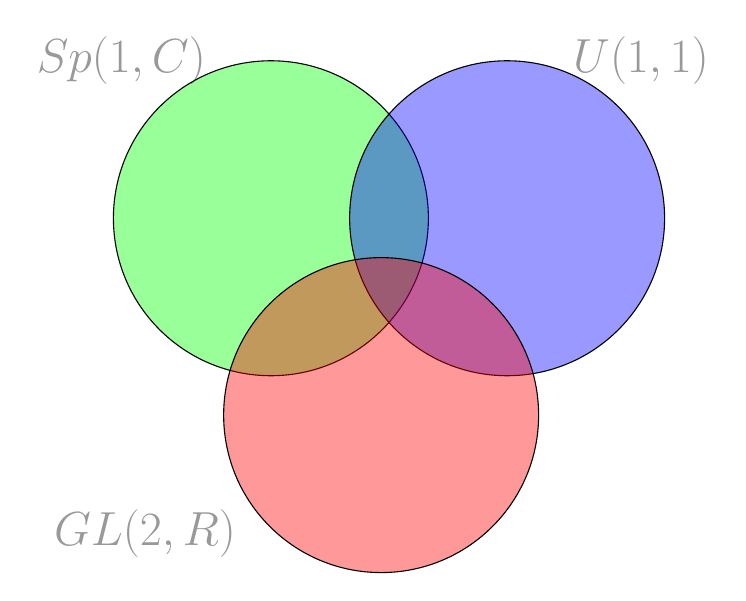
\begin{tikzpicture}
		%% You can adjust the opacity here. For venn diagrams it is convenient to have a low opacity so that you can see intersections
		\begin{scope} [fill opacity = .4]
			%% The draw command knows a lot of shapes. To make a rectangle you just need to specify two diagonal corners. Make sure you always have a semicolon at the end of your draw commands, otherwise latex flips out.
			%% Similarly, you can make a circle by specifying the center and then the radius. You can also add a fill color, but if you're printing in black and white you'll probably want to remove that line.
			\draw[fill=green, draw = black] (-1.4,1) circle (2);
			\draw[fill=blue, draw = black] (1.6,1) circle (2);
			\draw[fill=red, draw = black] (0,-1.5) circle (2);
			%% We can use the node command to label points. If you put your cursor on "LARGE" or "textbf" a box will drop down with size and text style options.
			\node at (-3.3,3) {\LARGE $Sp(1,\mathbb{C})$};
			\node at (3.3,3) {\LARGE $U(1,1)$};
			\node at (-3,-3) {\LARGE $GL(2,\mathbb{R})$};
		\end{scope}
		%% And now you have a venn diagram. Yay!
		%\draw[help lines](-5,5) grid (5,-6);    This line can draw the grid lines to help guide you. I use these when I'm writing the code and then delete this line when I publish the pdf.
	\end{tikzpicture}
\end{figure}
不难发现:
\begin{equation}
	Sp(1,\mathbb{C})\cap U(1,1)\cap GL(2,\mathbb{R})=SL(2,\mathbb{R})\cong SU(1,1)
\end{equation}
这其实就是$M$所在的集合,所以$M$很重要的一条性质是保$\left<\cdot,\cdot\right>$,也就是:\footnote{我们默认选取了$f_{1/2}$这组基底}
\begin{equation}
	M^\dagger I M =I,\quad I\equiv\operatorname{diag}(-,+)
\end{equation}
这直接导致$M$可以写成下面的形式:
\begin{equation}
	M=\begin{pmatrix}
		\alpha&\bar\beta \\
		\bar\beta&\bar\alpha
	\end{pmatrix},\quad |\alpha|^2-|\beta|^2=1
\end{equation}
现在考虑下面的$L_0$上的解,根据$M$是同构可以得知一定存在唯一的$L$中的解与之唯一对应:
\begin{equation}
	\psi_0=\begin{cases}
		f_1+r f_2&,x<x_1\\
		\tau f_1&,x>x_2
	\end{cases}
\end{equation}
只用证存在$M$使得$M\cdot (1,r)^\mathrm{T}=(\tau,0)^\mathrm{T}$即可,列出方程即可解得:
\begin{equation}
	r=-\frac{\beta}{\bar\alpha},\quad \tau=\frac{1}{\bar\alpha}
\end{equation}
其中$T\equiv|\tau|^2,R\equiv|r|^2$,他们之和为1,注意到由于$\alpha\neq 0$,所以无论如何体系都会有个非0的透射概率,当然反射概率可能为0。这和经典力学有很大的不同,经典力学透射必须要求$E>V_{\max}$。